% --- SYSTEM MODEL AND PROBLEM FORMULATION ---

\noindent This chapter describes the system model, formulates the task offloading problem mathematically, and provides a recap of the baseline M-DAFTO algorithm.

\section{System Model}

This work considers a healthcare IoT-fog system consisting of IoT devices and Fog Nodes (FNs), building upon the architecture defined in the M-DAFTO base model \cite{swain2024mdafto}. The IoT devices generate computational tasks, and the FNs process them. Figure~\ref{fig:system_model} illustrates this architecture.

\begin{figure}[htbp]
\centering
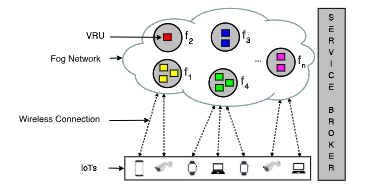
\includegraphics[width=0.85\textwidth]{Images/image1.png}
\caption{An IoT-Fog network comprising multiple IoT devices and FNs communicating over a wireless channel, adapted from \cite{swain2024mdafto}.}
\label{fig:system_model}
\end{figure}

\subsection{IoT Tasks}

Each IoT task $T_i$ (for $i = 1, 2, \ldots, M$) is characterised by:
\begin{itemize}
\item $\text{cpuDemanded}_i$: CPU demand in million cycles, drawn from $[210.0, 480.0]$ Mcycles.
\item $\text{inputSize}_i$: Input data size in KB, drawn from $[300.0, 600.0]$ KB.
\item $\text{outputSize}_i$: Output data size in KB, drawn from $[10.0, 20.0]$ KB.
\item $\text{deadline}_i$: Processing deadline in seconds, drawn from $[15.0, 22.0]$ s.
\item $\text{phase}_i$: Either ``Pre-Surgery'' or ``Post-Surgery'' (assigned randomly with equal probability).
\item $\text{severity}_i$: Either ``Major'' (critical operations) or ``Minor'' (routine tasks), assigned randomly with equal probability.
\end{itemize}

\subsection{Fog Nodes}

Each FN $F_j$ (for $j = 1, 2, \ldots, N$, where $N = 5$) is characterised by:
\begin{itemize}
\item $\text{totalCpuGHz}_j$: Total CPU capacity in GHz, drawn from $[6.0, 10.0]$ GHz.
\item $\text{numberOfVRUs}_j$: Number of Virtual Resource Units (VRUs), drawn from $[200, 500]$.
\item $\text{vruCapacity}_j = (\text{totalCpuGHz}_j \times 1000) / \text{numberOfVRUs}_j$ (Mcycles/s per VRU).
\end{itemize}

A VRU is a logical unit of compute capacity. A fog node with 400 VRUs can theoretically handle 400 concurrent tasks. The maximum quota of a fog node equals its number of VRUs.

\section{Problem Formulation}

\subsection{Offloading Delay}

For task $T_i$ offloaded to fog node $F_j$, the offloading delay is:
\begin{equation}
\text{delay}_{ij} = \text{txTime}_{ij} + \text{execTime}_{ij} + \text{rxTime}_{ij}
\end{equation}
where:
\begin{align}
\text{txTime}_{ij} &= \frac{\text{inputSize}_i}{\text{UPLINK\_DATA\_RATE}} \\
\text{execTime}_{ij} &= \frac{\text{cpuDemanded}_i}{\text{vruCapacity}_j} \\
\text{rxTime}_{ij} &= \frac{\text{outputSize}_i}{\text{DOWNLINK\_DATA\_RATE}}
\end{align}

The uplink and downlink data rates are both 2500.0 KB/s (derived from 20 MHz bandwidth).

\subsection{Energy Consumption}

The energy consumed when task $T_i$ is offloaded to fog node $F_j$ is:
\begin{equation}
\text{energy}_{ij} = (P_{\text{tx}} \times \text{txTime}_{ij}) + (P_{\text{exec}} \times \text{execTime}_{ij}) + (P_{\text{rx}} \times \text{rxTime}_{ij})
\end{equation}
where $P_{\text{tx}} = 0.5$ W (transmission power), $P_{\text{exec}} = 1.0$ W (execution power), and $P_{\text{rx}} = 0.5$ W (receiving power).

\subsection{Assignment Constraints}

A valid task assignment must satisfy:
\begin{itemize}
\item Each task is assigned to at most one fog node.
\item The number of tasks assigned to fog node $F_j$ must not exceed its maximum quota $q_j = \text{numberOfVRUs}_j$.
\item The number of tasks assigned to $F_j$ must meet its minimum quota $p_j$ (for fairness).
\item An unassigned task constitutes an \textit{outage}.
\end{itemize}

\section{Baseline M-DAFTO Recap}

The M-DAFTO algorithm \cite{swain2024mdafto} uses a Single-Type MSDA (Algorithm 9 from \cite{fragiadakis2016strategyproof}) with the following characteristics:

\subsection{2-Criteria Urgency Function}

For task $T_i$ at fog node $F_j$:
\begin{equation}
U(T_i, F_j) = w_1 \times \frac{1}{\text{deadline}_i - \text{delay}_{ij}} + w_2 \times \frac{1}{\text{pref}(T_i)}
\end{equation}
where $\text{pref}(T_i)$ is the number of fog nodes where $\text{delay}_{ij} \leq \text{deadline}_i$ (if 0, set to 1.0 to avoid division by zero), and $w_1, w_2$ are weights generated by a 2$\times$2 AHP matrix.

\subsection{2$\times$2 AHP Weight Generation}

M-DAFTO generates weights using a 2$\times$2 pairwise comparison matrix. With only 2 criteria, the matrix always passes the consistency check (CR = 0 by definition), providing no actual validation.

\subsection{Quota Determination}

Minimum quotas are computed proportionally based on VRU capacity relative to the most efficient node. For each fog node $F_j$:
\begin{equation}
p_j = \min\left(\left\lfloor \frac{\text{vruCapacity}_j}{\lambda_{\max}} \times l_{\max} \right\rfloor, \; \text{numberOfVRUs}_j\right)
\end{equation}
where $\lambda_{\max}$ is the maximum VRU capacity across all fog nodes, and $l_{\max} = \min(h_{\max}, \lfloor |T| / |F| \rfloor)$ with $h_{\max}$ being the number of VRUs of the most efficient node. Maximum quotas equal the number of VRUs.

\subsection{Time Complexity}

M-DAFTO achieves a time complexity of $O(m \cdot n)$ per DA round, where $m$ is the number of tasks and $n$ is the number of fog nodes \cite{swain2024mdafto}.